\chapter*{Sample Section}

\section{This is a section}

    \subsection{This is a subsection}
        
        \subsubsection{This is a subsubsection}

            Note that subsubsection will not be included in the table of cotents.
            
            Text.\\ %\\to start a new line
            \verb!\\to start a new line!
            
            A better practice when writing long sections is to start a new \emph{paragraph}.
            
            Emphasise: use \emph{normal emph} (\verb!\emph{normal emph}!), self-defined \empha{red emph} (\verb|\empha{red emph}|, and self-defined \emphb{blue emph} (\verb|\emphb{blue emph}|). Typically, I use the blue emph to highlight \emphb{new concepts} (\verb|\emphb{new concepts}|) in main lines.
            
            \textbf{Bold text} (\verb|\textbf{Bold text}|)
            
            \textit{Italic text} or \emph{Italic Text} (\verb|\textit{Italic text}|)
            
            \textcolor{red}{Coloured text} (\verb|\textcolor{red}{Coloured text}|)
            
            Inline equation:$x+y=z$ (\verb!$x+y=z$!)
            
            Displayed equation:
            \begin{itemize}
                \item coloured equation (\verb!$$\color{red} x+y=z$$!)$$\color{red} x+y=z$$  
                \item fraction (\verb|$$\frac{1}{a}$$|)$$\frac{1}{a}$$
                \item summation (\verb|$$\sum_{i=1}^{T}$$|)$$\sum_{i=1}^{T}$$
                \item special notations $$\infty \partial$$
                \item greek letters $$\alpha \beta \gamma \sigma \delta \phi \psi \epsilon$$
                \item arrows $$\rightarrow \Rightarrow$$
                \item underbrace (\verb|$$\underbrace{expression}_{text}$$|)$$\underbrace{expression}_{text}$$
                \item max (\verb|$$\max_{\alpha} x+y$$|)$$\max_{\alpha} x+y$$
                \item relations (\verb|$$\approx > \neq \geq \leq$$|)$$\approx > \neq \geq \leq$$
                \item Tilde/hat $$\Tilde{\alpha} \hat{\alpha}_i^2 \times X$$
            \end{itemize}

            Displayed equation with reference label (\verb|\label{} or \tag{} under \begin{equation}| label for reference, tag for display):
            \begin{equation}
                \color{blue}%you can set a color. My practice is to colour important equations red.
                \label{eqn:1}%set a label for reference. No need to label if you don't want to refer to it later
                \tag{Equation Tag}%delete this line if you want to use auto-generated number
                x+y=z
            \end{equation}

            Unordered list:
            \begin{itemize}
                \item item 1
                \item item 2
            \end{itemize}
            
            Ordered list:
            \begin{enumerate}
                \item item 1
                \item item 2
            \end{enumerate}
            
            Insert figure:
            \begin{figure}[H]%option [H] means "strictly here"
                \centering
                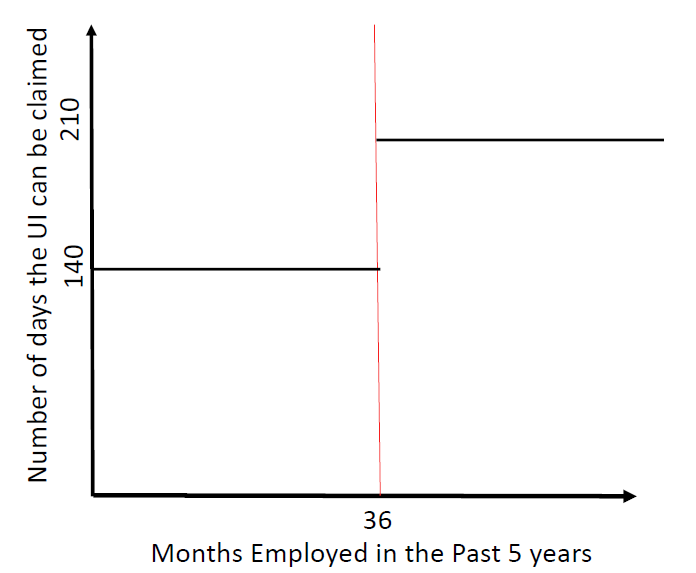
\includegraphics[width=2in]{images/ch1/card_1.png}%[scale option]{path and file name of the figure}
                \caption{an example}%caption
                \label{fig:label}%label for referencing. No need to include this if you don't need to refer back
            \end{figure}
Code:\\
\verb|\begin{figure}[H]%option [H] means "strictly here"|\\
\verb|\centering|\\
\verb|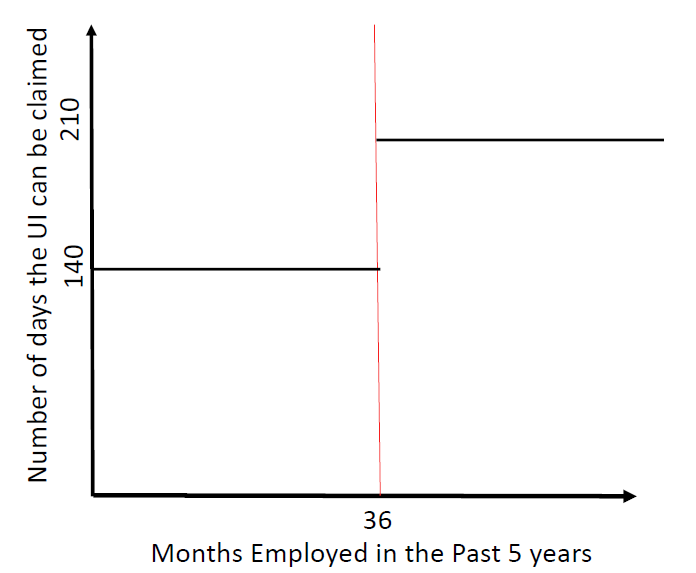
\includegraphics[width=2in]{images/ch1/card_1.png}%[scale option]{path and file name}|\\
\verb|\caption{an example}%caption|\\
\verb|\label{fig:label}%label for referencing. No need to include this if you don't need to refer back|\\
\verb|\end{figure}|









\section{123123}


    \begin{itemize}
        \item this is an item
        \item this is another item
        \begin{itemize}
            \item another
        \end{itemize}
    \end{itemize}

    \begin{enumerate}
        \item 12
        \item sjaiwjiodajo
    \end{enumerate}

    \begin{equation}
        x+y
    \end{equation}

    \begin{equation*}
        x+y
    \end{equation*}

    $$x+y$$

    this fraction $\frac{a}{b}$

    \begin{figure}[H]
        \centering
        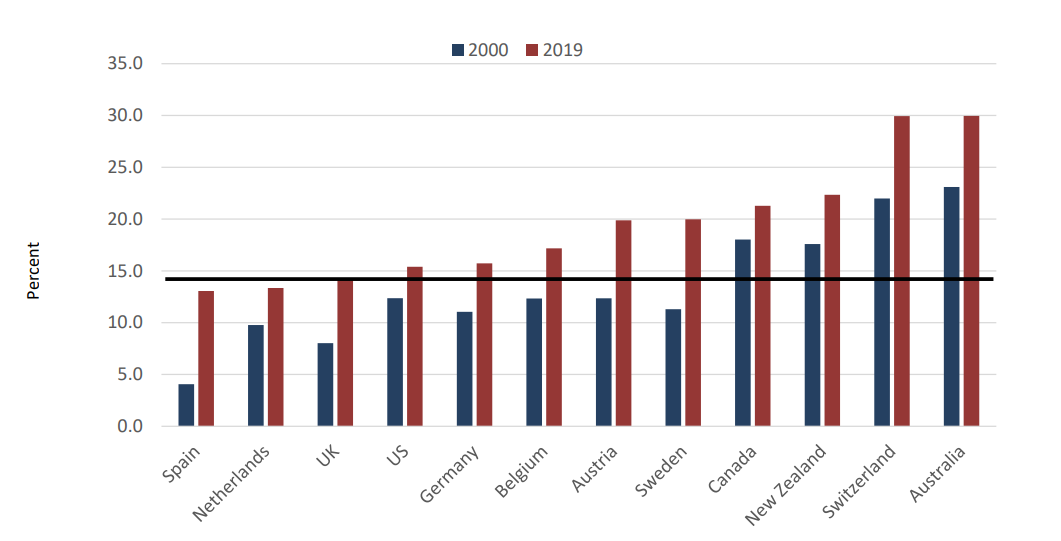
\includegraphics[width=4.5in]{images/ch11/2.png}
        \caption{This is a graph}
        \label{123123}
    \end{figure}

    \ref{123123}